\documentclass[12pt,letterpaper,english]{article}
\usepackage[utf8]{inputenc}
\usepackage[T1]{fontenc}
\usepackage[english]{babel}
\usepackage[letterpaper, margin=1in]{geometry}
\usepackage[pdftex]{graphicx}
\usepackage{fancyhdr}
\usepackage{setspace}
\usepackage{amsmath}
\usepackage{commath}
\usepackage{lastpage}
\usepackage[usenames,dvipsnames,svgnames,table]{xcolor}
\usepackage{minted}
\usepackage{isodate}
\pagestyle{fancy}
\fancyhead{}
\fancyfoot{}
\fancyhead[HR]{\thepage\ of \pageref{LastPage}}

\begin{document}


\begin{titlepage}
\thispagestyle{plain}
\begin{center}
\topskip0pt
\vspace*{\fill}

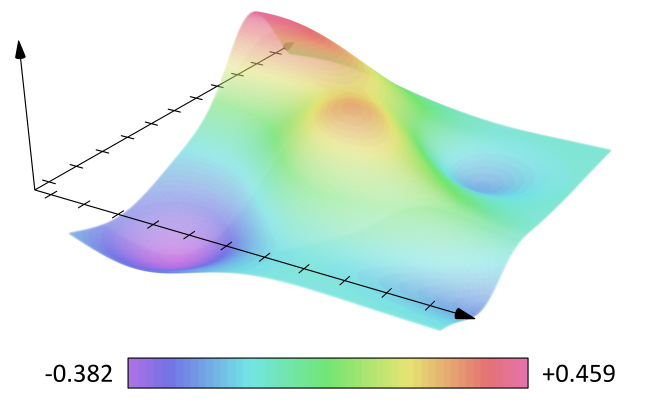
\includegraphics[width=3cm]{logo.png}~\\[1cm]

\rule{\linewidth}{0.5mm}\\[0.5cm]

\textsc{\LARGE Visualizing functions of multiple variables}\\[1cm]

\textsc{\large By Sam Grayson and Wilson Nguyen}\\[0.7cm]

{\large \isodate Version 0.1} \\[0.7cm]

\rule{\linewidth}{0.5mm}\\[1cm]

\vspace{0.9cm}

\end{center}

\section*{Abstract}

Visualizing the concepts of multivariable calculus can be challenging. The students created several computer-generated visual models utilizing the Mathematica language. These models can be used as teaching aids for educators or extra instruction for students.

\vspace*{\fill}

\end{titlepage}

\section*{Acknowledgements}

Thank you to Mrs. Harrelson for making a remarkable Multivariable Calculus class at LASA. This class is seriously the bomb if you like to think mathematically. We want to acknowledge the families of the students who have been incredibly supportive, even though they don't understand why we are doing this.

\tableofcontents

\clearpage

\doublespacing

\section{Introduction}

 As students, we know that visualizing these topics can sometimes be pretty difficult. I may or may not be guilty, on occasion, of simply using these formulas without an understanding of what they really do. If only there were some means of playing around with these topics without having to imagine clear mountains with magical rings or bleeding, toilet paper pasted shaved faces (inside joke). We believe that we have created the solution!

 The magic of Multivariable can be seen through the “Sam and Wilson’s 3D Multivariable Visualizer for Glazed-eyed LASA students” for a small fee of appreciation. The goals of this Visualizer are to allow students to interact with the topics discussed below and instead of telling the students  what the topics are, the Visualizer simply shows them. The topics would reveal themselves to even the most distant of students simply nodding their heads as asked (inside joke once more). We hope that you incorporate this Visualizer into your lessons and take advantage of the many opportunities that this opens up for students.

\section{Design Principles}

\begin{itemize}
\item \textbf{Flexibility:} The same concept can be visualized on multiple examples, and we tried to make it so that the models can adjust at runtime to any user inputted example.
\item \textbf{Interactivity:} The concepts are best illustrated when the user can tweak the values and adjust the parameters in a dynamic way that gives real-time feedback.
\item \textbf{Maintainability:} The models \textit{look good}. They are designed to be very clean and adjustable. This means that the code may be less aligned with the mathematics, but it is worth it for ease of maintaining. This way, when we graduate the models may still be adapted to the curriculum.
\item \textbf{Instructiveness:} The models are not by themselves. They are accompanied by text % TODO: in this paper?
explaining how they work and what they do.
\end{itemize}

\section{Frenet-Serret frames}

\subsection*{Overview}

The Frenet frame is a tool for understanding the local motion of a curve. The Frenet-Serret frame gives you an idea of where the function would be going if it were a straight line (tangent vector), which way the function would be bending if it were a circle (normal vector), and which way the function is twisting (binormal vector). Additional quantities like the curvature (related to the radius of the function if it were a circle) and the torsion (related to the angular momentum in the direction of the binormal vector). This visualization renders a video which shows the Frenet-Serret frame moving along a path. \cite{frenet1} \cite{frenet2} \cite{frenet3}

\subsection*{Theoretical basis}

The input should be a regular path in real space. \(c(t) : [a, b] \to \mathrm R^3\).

\begin{enumerate}
%\item Unit parametrize the curve. Let the arc-length passed up as a function of time given by \(s(t)\) \(s(t) = \int\limits_0^t \|f'(t)\|\). It can be shown that \(s(t)\) always has an inverse \(s^{-1}(t)\) (See the appendix for proof). Then let \(f(s^{-1}(t)) = c(t)\).
% TODO: link to appendix

%Since \(s'(t) = \|f'(t)\|\) by the fundamental theorem, and the length of a vector must be positive, the \(s(t)\) must be monotonically increasing. All monotonically increasing functions are injective. Taking \(\cod f = \im f\), it must also be surjective. Therefore \(s(t)\) is always invertible.

\item Calculate the unit tangent vector. Taylor's Theorem gives us \(c(t_0) + c'(t) \cdot (t - t_0) \approx c(t)\) for small \(\delta t\). A straight line starting at \(\vec{u}\) in the direction of \(\vec{v}\) is given by \(\vec{u} + \vec{v} \cdot t\). Therefore the line that locally approximates the function \(f\) is the first-order Taylor's Theorem. Since the tangent vector is relative to the point\(\vec{u} = \vec{0}\), and relative to the time \(t = 0\), and unit normalized, it is given by \(T(t) = \frac{c'(t)}{\|c'(t)\|}\).

\item Calculate the unit normal vector. Let \(c(t)\) be approximated by a circle of radius \(r\) lying in the plane spanned by \(T(0)\) and \(N(0)\) (this vector is not yet known). \(c(t) \approx r T(0) \sin t + r N(0) \cos t\). Then \(c'(t) = r T(0) \cos t - r N(0) \sin t\) (the reader can verify that at \(t = 0\), the tangent vector is indeed \(T(0)\)). Then \(c''(t) = T'(t) = - r T(0) \sin t - r N(0) \cos t\). Therefore \(T'(0) = -rN(0)\) which points in the direction of the normal vector. Therefore the unit-normalized normal vector is given by \(N(t) = \frac{T'(t)}{\|T'(t)\|}\). % TODO: get rid of negative sign

\item Calculate the curvature. \(\kappa(t) = \frac{1}{r}\) in the circle described by \(c(t) \approx r T(0) \sin t + r N(0) \cos t\). As previously shown, \(T'(0) = -r N(0)\). Therefore \(\frac{1}{\|T'(0)\|}\) gives the curvature.

% TODO: explain torsion

\item Calculate the binormal vector. In order to form an orthnormal basis, \(B(t) = T(t) \times N(t)\).

%\item Additionally, the Darboux vector can be computed. The Darboux vector is the angular velocity vector. The rate of rotation going from one vector to another is the cross-product between the vectors divided by the time it took to rotate. Therefore % TODO: complete this

\end{enumerate}

\subsection*{Implementation details}

There are multiple ways the Wolfram Language can compute derivatives. The first is \href{https://reference.wolfram.com/language/ref/D.html}{symbolically computing the derivative}. This calculates the answer using the variables. \(\frac{\dif}{\dif x}(3x^2)\) could be written \verb+D[3x^2, x]+ which evaluates to \verb+6x+. This expression can later be evaluated with a specific \verb+x+ for a numeric answer. The second is \href{http://reference.wolfram.com/language/NumericalCalculus/ref/ND.html}{numerically computing the derivative}. This method uses a very small change in the independent variable. \(\frac{\dif}{\dif x}(3x^2\mid_{x=5})\) could be written \verb+ND[3x^2, x, 5]+ evaluates to \verb+30+. There are functions like the absolute value which don't have symbolic derivatives, but do have numeric derivatives. It is also about ten times faster. Therefore, for this program I used the numeric derivative.

All of the important quantities are given as a function of \verb+t+. This is because it makes animation easier if arbitrary inputs can be supplied. First the user enters a path as a function of \verb+t+. Then the tangent vector (based on the path), the normal vector (based on the tangent vector), and the binormal vector (based on the tangent and normal vectors) are calculated as described in previous subsection. The curvature is calculated based on the tangent vector, as described in the previous subsection.

After that each quantity described above must be rendered as a 3D-graphic. The output is put into a single frame. Outputs from different points along the path are put into a list. That list gets animated by the built-in \href{https://reference.wolfram.com/language/ref/ListAnimate.html}{ListAnimate}.

\subsection*{Usage notes}

This program could be used to create a video demonstrating the Frenet-Serret frames in preparation for a lecture (not real-time). This video could be displayed after slide 4 of lecture 6 (Motion in 3 space). It would provide a visualization for what the Frenet-Serret frame represents.

\begin{enumerate}
\item Change \verb+pathF[t_] = ...+ to be whatever path you want in terms of \verb+t+.
\item Change \verb+tmin+ and \verb+tmax+ to span the domain of the path.
\item Evaluate the cell with Shift+Enter. You should see a the path appear below. Tweak any of the above values if necessary.
\item Evaluate each cell until you hit the bottom with Shift+Enter. It may take up to twenty minutes to render the video.
\item When completed, the Wolfram Language should display a file name in the last cell. The video is located there.
\end{enumerate}


\end{document}
